\subsection{Optimizing the Common Research Model Wing}
\label{ch5:sec:cs2}

We now turn to NASA's Common Research Model Wing (CRM wing), which is extracted from the CRM wing-body configuration. As shown in Fig.~\ref{ch5:fig:cs2_template_mesh}(b), the initial geometry is a 3D wing with a blunt trailing edge. As in the previous case, results are compared to those obtained with the FFD baseline.

\subsubsection{Problem Formulation}

The objective is to minimize the drag coefficient $C_D$ while maintaining a lift coefficient $C_L$ of $0.5$ and ensuring that the pitching moment coefficient $C_M$ is at least $-0.17$. This single-point optimization problem is conducted under fully turbulent flow conditions, with a Mach number of $0.85$, a Reynolds number of $5 \times 10^6$, and an initial angle of attack of $2.2^{\circ}$. Additional constraints require the wing's volume to remain at least as large as its initial value, and its thickness to be no less than $25\%$ of the initial thickness. The trailing edge (TE) vertices and the leading edge (LE) vertex on the root section are fixed, while the remaining LE vertices are restricted to movement along the $z$ direction, preserving the projected area.
The optimization objectives and flow conditions follow the ADODG-4.1 single-point optimization benchmark~\footnote{\url{https://sites.google.com/view/mcgill-computational-aerogroup/adodg}}.

The optimization is performed on a grid with $450,560$ cells, as shown in Fig.~\ref{ch5:fig:cs1_template_mesh}(a), which corresponds to the L2 grid defined in~\citet{aa.Lyu2015}. In this setup, the DeepGeo weights affect only the wing’s surface shape, while the angle of attack is treated as a standalone design variable. Tab.~\ref{ch5:tab:crm_DV_cons} summarizes the experimental setup.

\begin{figure}[!tb]
    \begin{center}
        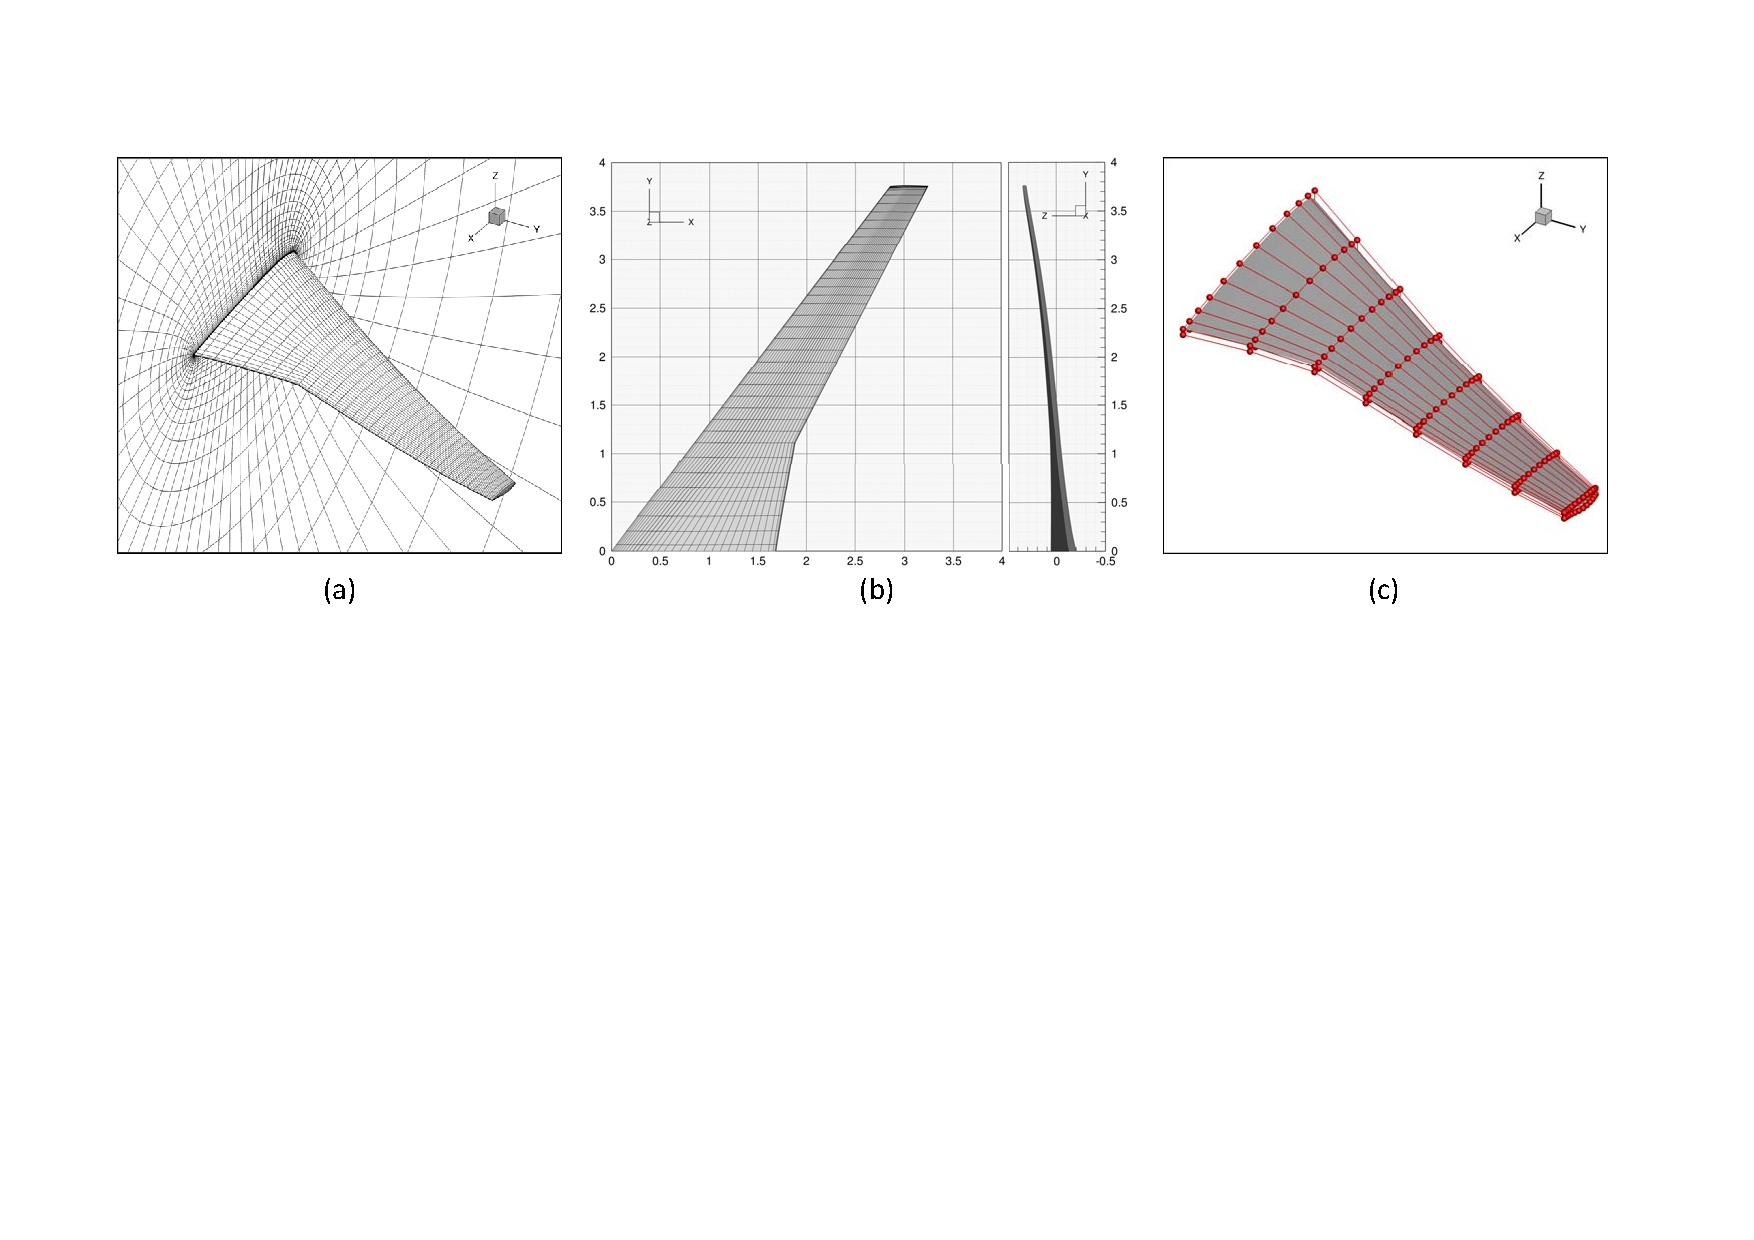
\includegraphics[width=1\linewidth]{chapter5/fig/crm_template_mesh_initial_geometry.pdf}
    \end{center}
    \caption{
        \small The geometric setups for Case Study II, including: (a) the template mesh for DeepGeo, (b) the initial CRM wing geometry and (c) the 192-point FFD setting.
    }
    \label{ch5:fig:cs2_template_mesh}
\end{figure}

\subsubsection{Configuring DeepGeo}

As in the previous case study, the L2 grid is used as the input template mesh $\hat{M}$.
The objective function $\cO_{CFD}$ and the loss function $\cL_{cons}$ from Eq.~\ref{ch5:eq:asoObj} are defined as:
%
\begin{align}
    \cO_\text{CFD} & = \left| C_D \right| + \left| C_L-0.5 \right| + \max \left( -0.17 - C_M, 0 \right) \;, \label{ch5:eq:cfdWing}  \\
    \cL_{cons} & = 
    \underbrace{{\max \left(Vol(V^S)-{Vol}_\text{original}(S), 0\right)} ^2}_\text{volume constraint} + 
    \underbrace{\left|\left|\Delta V^\text{TE}\right|\right|^2}_\text{TE constraint} +
    \underbrace{\left|\left|\Delta V^\text{LE}_x\right|\right|^2 + \left|\left|\Delta V^\text{LE}_y\right|\right|^2}_\text{LE constraint} +
    \underbrace{\left|\left|\delta \bv^\text{LE,root}\right|\right|^2}_{ \substack{\text{fixed-wing root}\\ \text{incidence constraint}} } \; . \nonumber
\end{align}
%
Minimizing $\cO_{CFD}$ aims to reduce $C_D$, bring $C_L$ close to 0.5, and ensure $C_M$ is greater than or equal to $-0.17$.  The extended Shoelace formula~\cite{aa.Zhang2001} is applied to compute the volume $Vol(V^S)$ of the deformed wing, with an arbitrary reference point on the root section plane. ${Vol}_\text{original}(S)$ represents wing's initial volume. The term $\bv^\text{LE,root}$ corresponds to the single leading-edge (LE) vertex on the root section, while $V_x$ and $V_y$ refer to the sets of $x$ and $y$ vertex coordinates, respectively. In practice, DeepGeo satisfies the thickness requirement without an explicit loss function term.

\begin{table}[!t]
  \centering
  \caption{\small Aerodynamic shape optimization task specifications for the Case Study II.}
  \resizebox{1\columnwidth}{!} {
        \begin{tabular}{lllrr}
        \hline
        \multicolumn{1}{l}{\textbf{Objectives}} & \textbf{Functions/Variables} & \textbf{Description} & \multicolumn{1}{l}{\textbf{DeepGeo Quantity}} & \multicolumn{1}{l}{\textbf{FFD Quantity}} \\
        \hline
        \multicolumn{1}{l}{\textbf{Minimize}} & $C_D$  & Drag coefficient &        &  \\
        \hline
        \multicolumn{1}{l}{\multirow{3}[2]{*}{\textbf{With respect to}}} & $\Theta$ & Weights of DeepGeo & \num{151585} &         \\
        \multicolumn{1}{l}{} & $P_z$  & Control points' $z$ coordinates &        & 720 \\
        \multicolumn{1}{l}{} &   & Twist function &        & 7 \\
        \multicolumn{1}{l}{} & $\alpha$ & Angle of attack & 1      & 1 \\
        \hline
        \multicolumn{3}{l}{\textbf{Total design variables}} & \num{151586} & 728 \\
        \hline
        \multicolumn{1}{l}{\multirow{9}[2]{*}{\textbf{Subject to}}} & $C_L=0.5$ & Lift coefficient constraint & 1      & 1 \\
        \multicolumn{1}{r}{} & $C_M\geq-0.17$ & Moment coefficient constraint & 1      & 1 \\
        \multicolumn{1}{r}{} & $t \ge 0.25 \; t_\text{original}$ & Minimum thickness constraints &        & 750 \\
        \multicolumn{1}{r}{} & $Vol \ge {Vol}_\text{original}$ & Minimum volume constraint & 1      & 1  \\
        \multicolumn{1}{r}{} & $\Delta V^\text{TE}=0$ & Trailing edge constraint & 1      &  \\
        \multicolumn{1}{r}{} & $\Delta V^\text{LE}_x=0,\;\Delta V^\text{LE}_y=0$ & Leading edge constraint & 1      &  \\
        \multicolumn{1}{r}{} & $\delta\bv^{\text{LE,root}}=0$ & Fixed-wing root incidence constraint & 1      &  \\
        \multicolumn{1}{r}{} & $\Delta P^{\text{TE,upper}}_z = -\Delta P^{\text{TE,lower}}_z$ & Fixed trailing-edge constraints &        & 15 \\
        \multicolumn{1}{l}{} & $\Delta P^{\text{LE,upper,root}}_z =$ & \multirow{2}[1]{*}{Fixed-wing root incidence constraint} & \multirow{2}[1]{*}{} & \multirow{2}[1]{*}{1} \\
        \multicolumn{1}{l}{} &  $\;\;\;-\Delta P^{\text{LE,lower,root}}_z$ &        &        &  \\
        \multicolumn{1}{r}{} & $2.0 \leq \alpha \leq 4.0$ & Angle of attack constraint & 1      &  1 \\
        \hline
        \multicolumn{3}{l}{\textbf{Total constraints}} & 7      & 770 \\
        \hline
        \multicolumn{3}{l}{\textbf{Need value range limits for each DV?}} & NO     & YES \\
        \hline
        \end{tabular}%
    }
  \label{ch5:tab:crm_DV_cons}%
\end{table}%

\subsubsection{Configuring the Free-Form Deformation Baseline}

For comparison, we use the FFD-based baseline with 192-control-point configuration of \citet{aa.Hwang2019,aa.Li2019}, as depicted in Fig.~\ref{ch5:fig:cs2_template_mesh}(c). Let the control points be $P=\{\bp_1, \bp_2,..., \bp_{192}\}$, where each $\bp=\{p_x, p_y, p_z\}$ and their displacements denoted as $\Delta P$. The positions of control points are optimized, and the wing's surface is interpolated within each control cages to enable localized shape changes. Additionally, a global function is implemented to introduce spanwise twisting, with seven rotation angles treated as additional design variables.
The 192 control points are grouped into seven sections along the wingspan and each section is rotated independently.
For this optimization, we use the MACH-Aero framework, where pyGeo~\cite{aa.Kenway2010} implements the FFD parameterization, IDWarp~\cite{aa.Secco2021} deforms the computational mesh and pyOptSparse~\cite{aa.Wu2020} for optimization.

\subsubsection{Results and Analysis}

\begin{table}[!b]
  \centering
  \caption{\small CRM wing optimization results of the Case Study II. One count for $C_D$ equals to $10^{-4}$.}
    \begin{tabular}{lcccc}
    \hline
    \textbf{Parameterization} &  \multicolumn{1}{l}{\textbf{Final} $C_D$ {\footnotesize(counts)}} & \multicolumn{1}{l}{\textbf{Final} $C_L$} & \multicolumn{1}{l}{\textbf{Final} $C_M$} & \multicolumn{1}{l}{\textbf{Final} $\alpha$}\\
    \hline
    \textbf{DeepGeo} & \num{200.05}  & \num{0.5000}  & -0.1717  & 2.08 \\
    \textbf{FFD} & \num{199.03}  & \num{0.5000}  & -0.1700  & 2.14 \\ 
    \hline
    \end{tabular}%
  \label{ch5:tab:crm_result}%
\end{table}%

\begin{figure}[!t]
    \begin{center}
        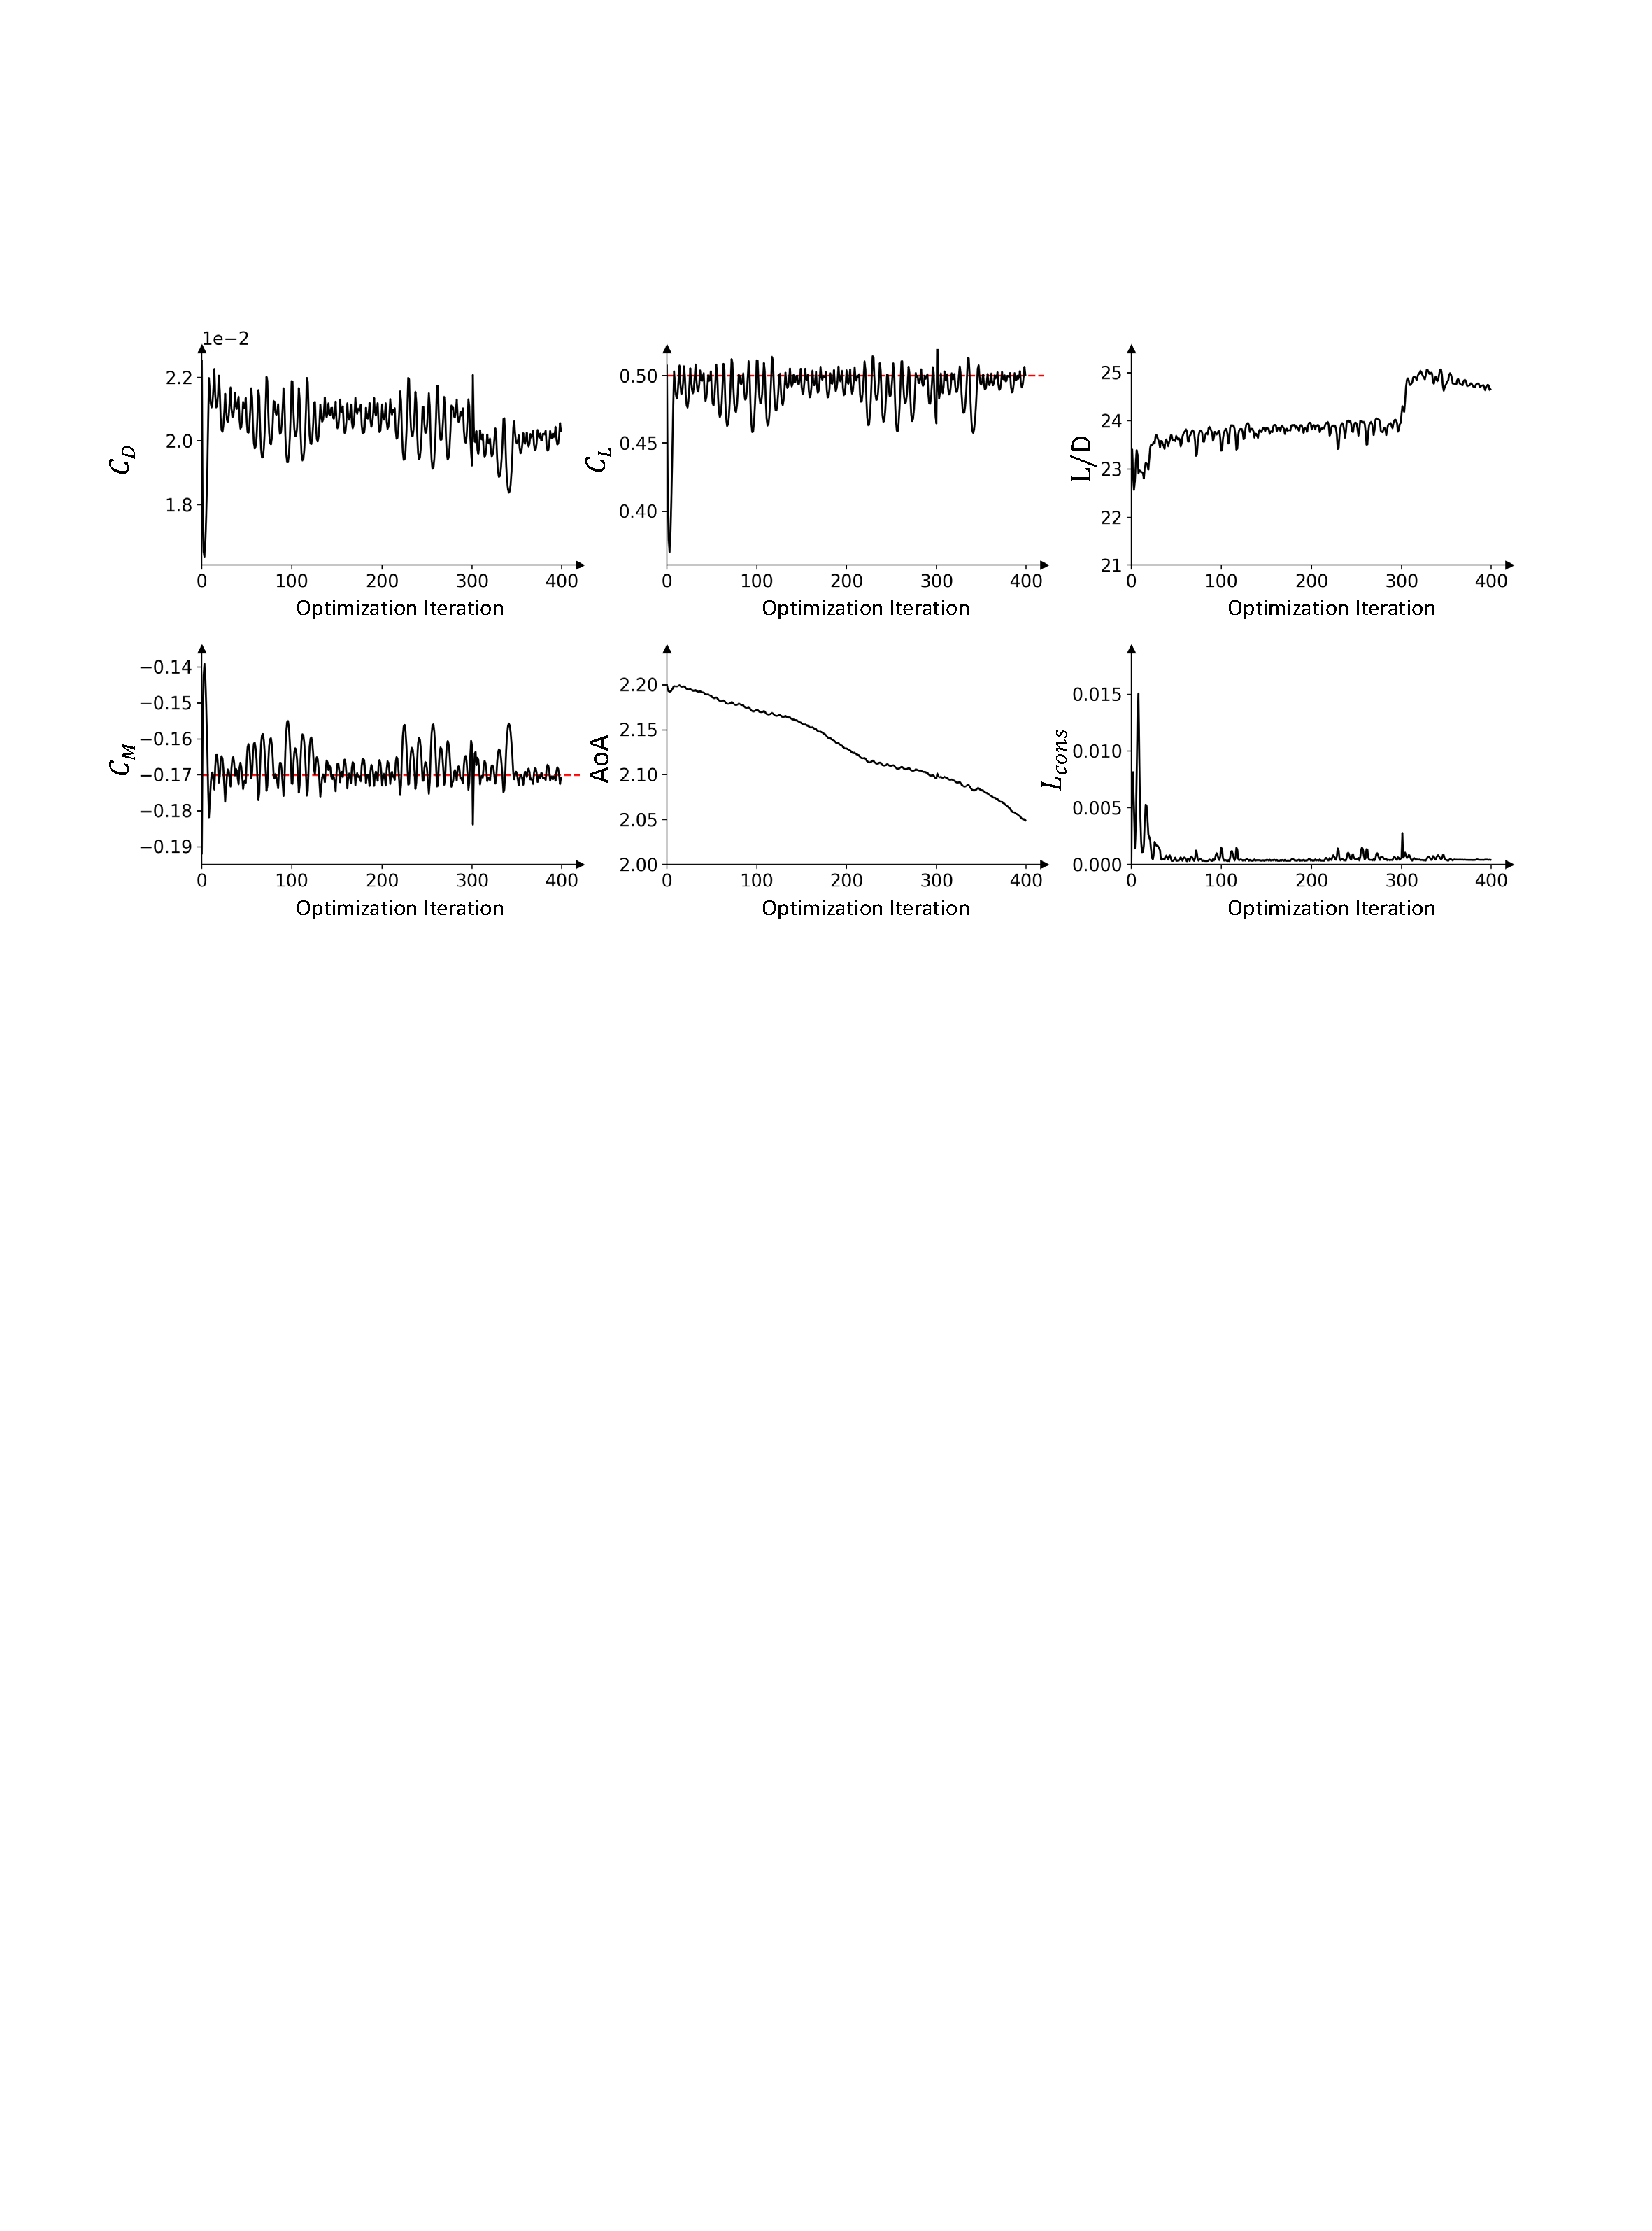
\includegraphics[width=1\linewidth]{chapter5/fig/crm_optim_history.pdf}
    \end{center}
    \caption{
        \small The optimization history of Case Study II. The dashed line in $C_L$ and $C_M$ figures demonstrates the optimization objectives.
    }
    \label{ch5:fig:cs2_history}
\end{figure}

\begin{figure}[!t]
    \begin{center}
        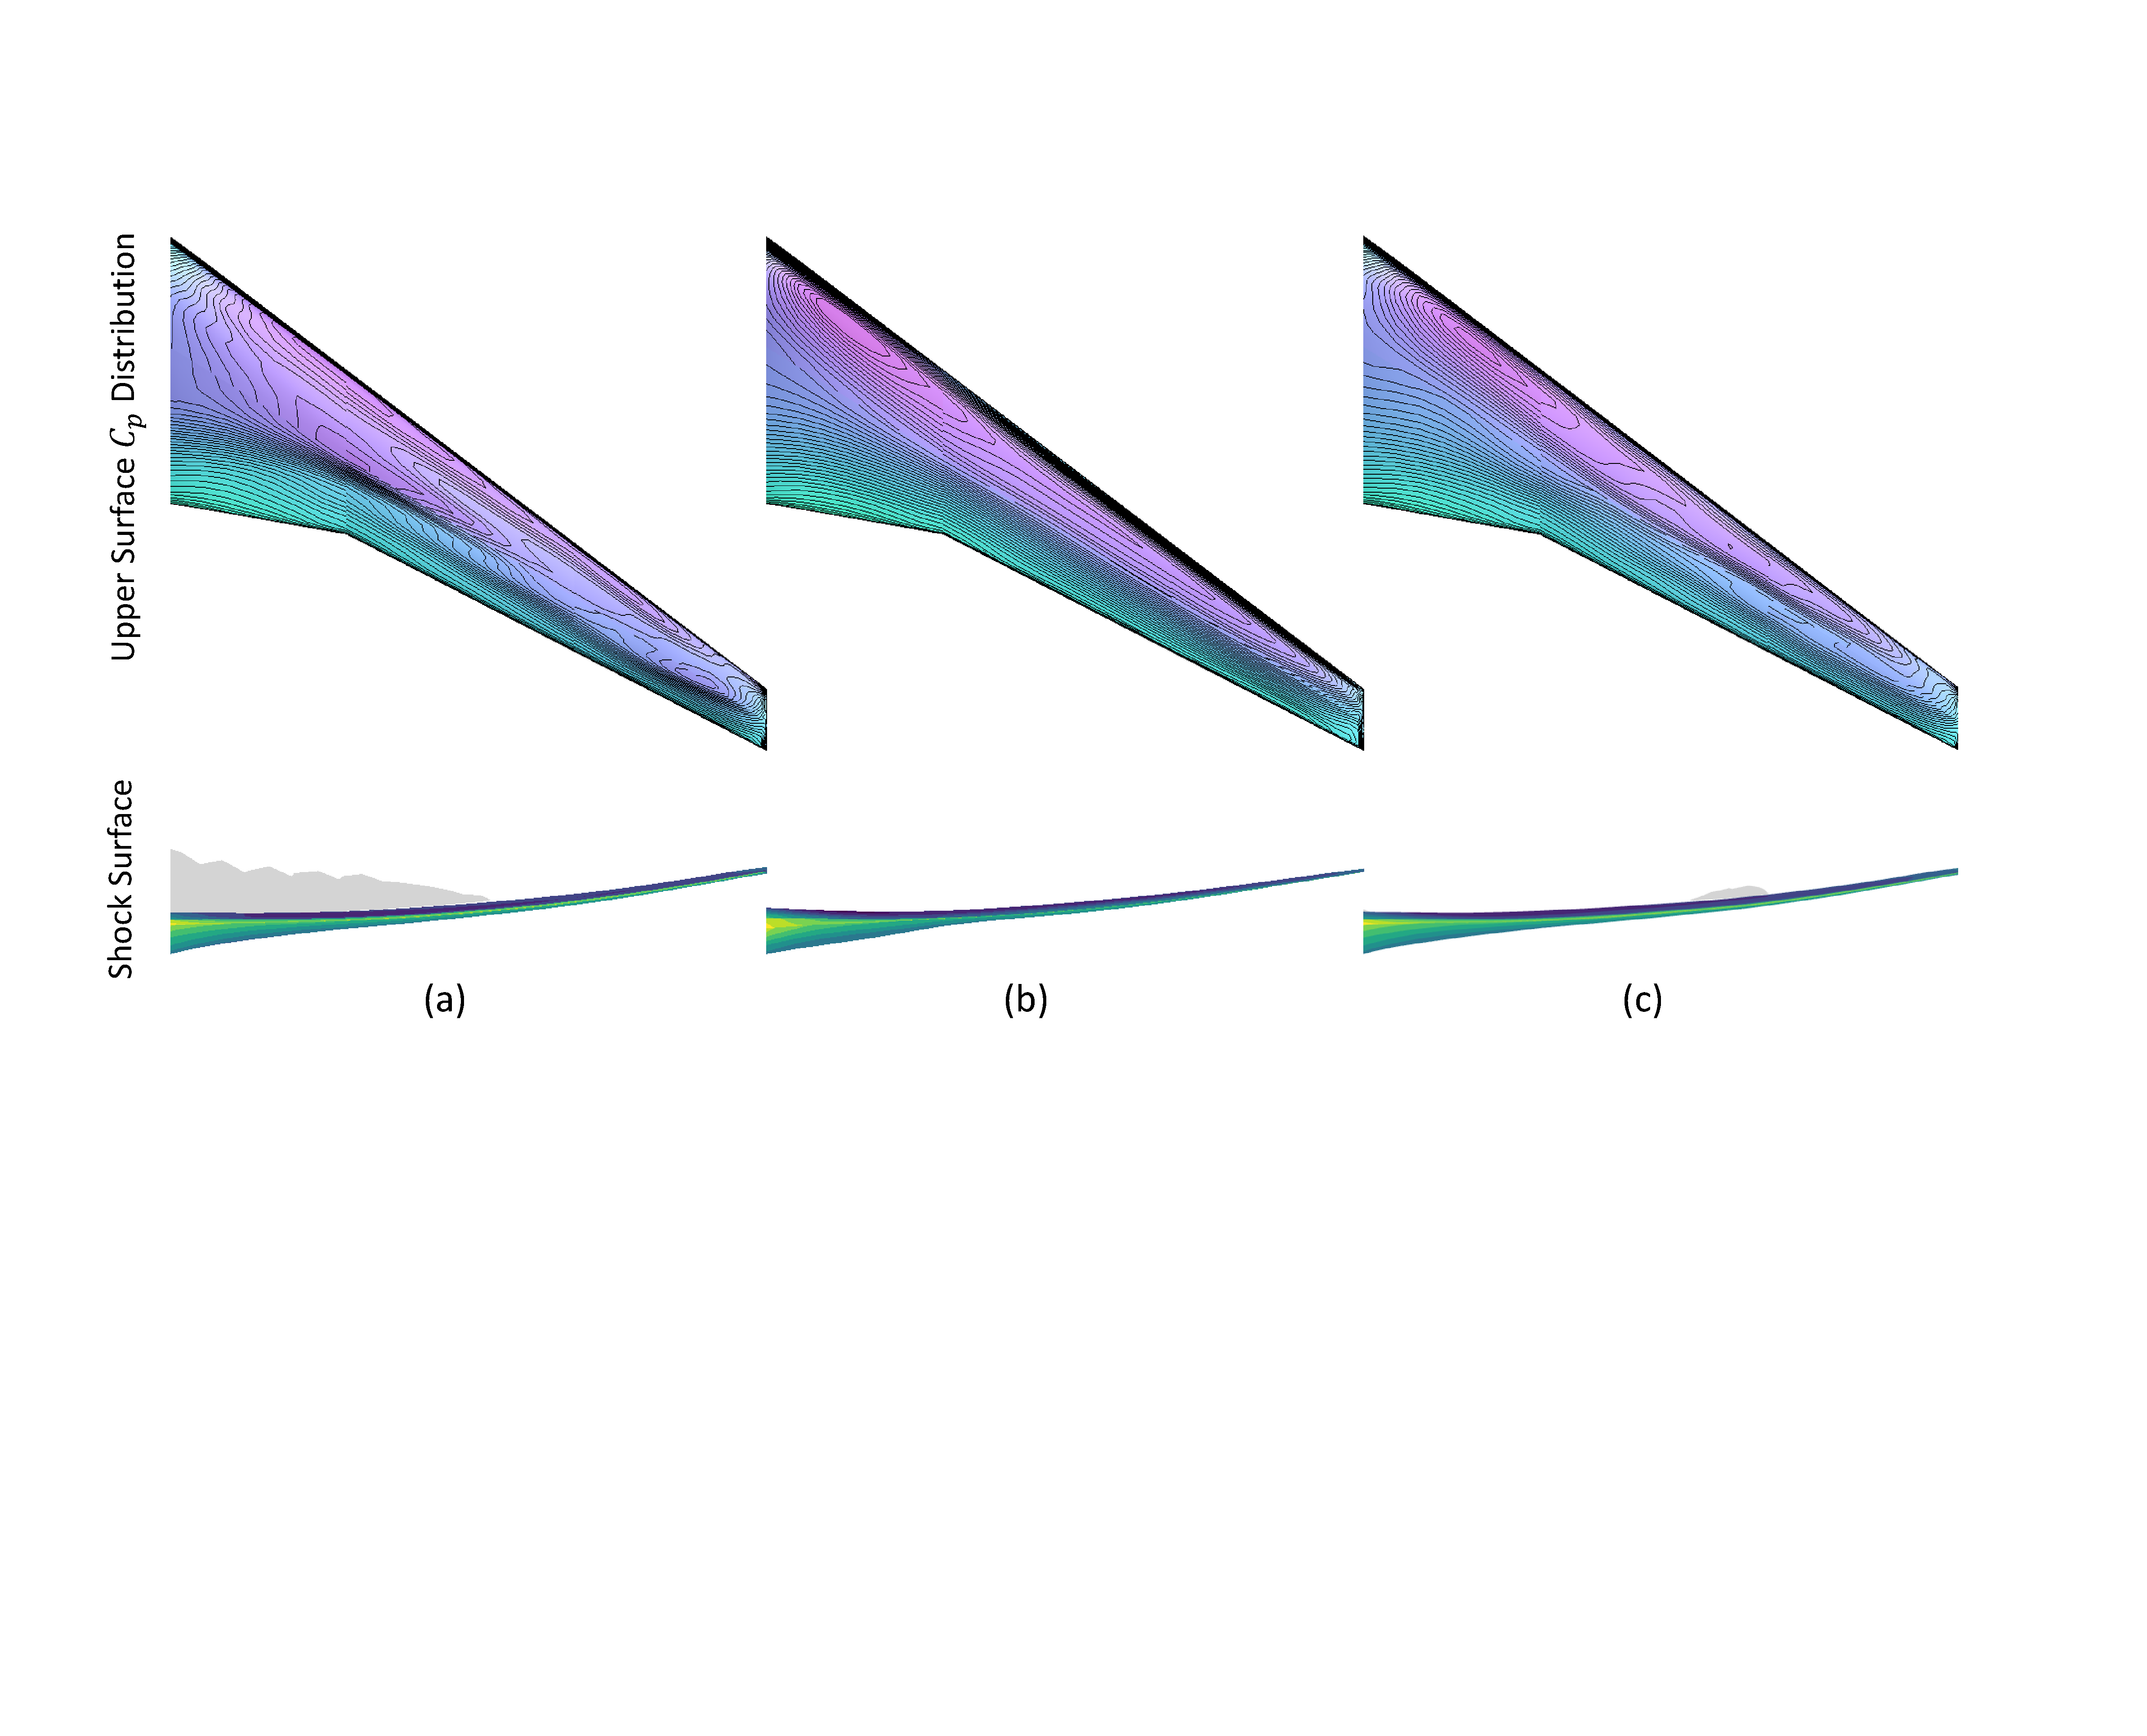
\includegraphics[width=1\linewidth]{chapter5/fig/crm_optim_cp.pdf}
    \end{center}
    \caption{
        \small A comparison of Case Study II on the pressure coefficient distributions and shock shapes of (a) the initial CRM wing, (b) the wing optimized with 192-point FFD, and (c) the wing optimized with DeepGeo.
    }
    \label{ch5:fig:cs2_cp}
\end{figure}

\begin{figure}[!h]
    \begin{center}
        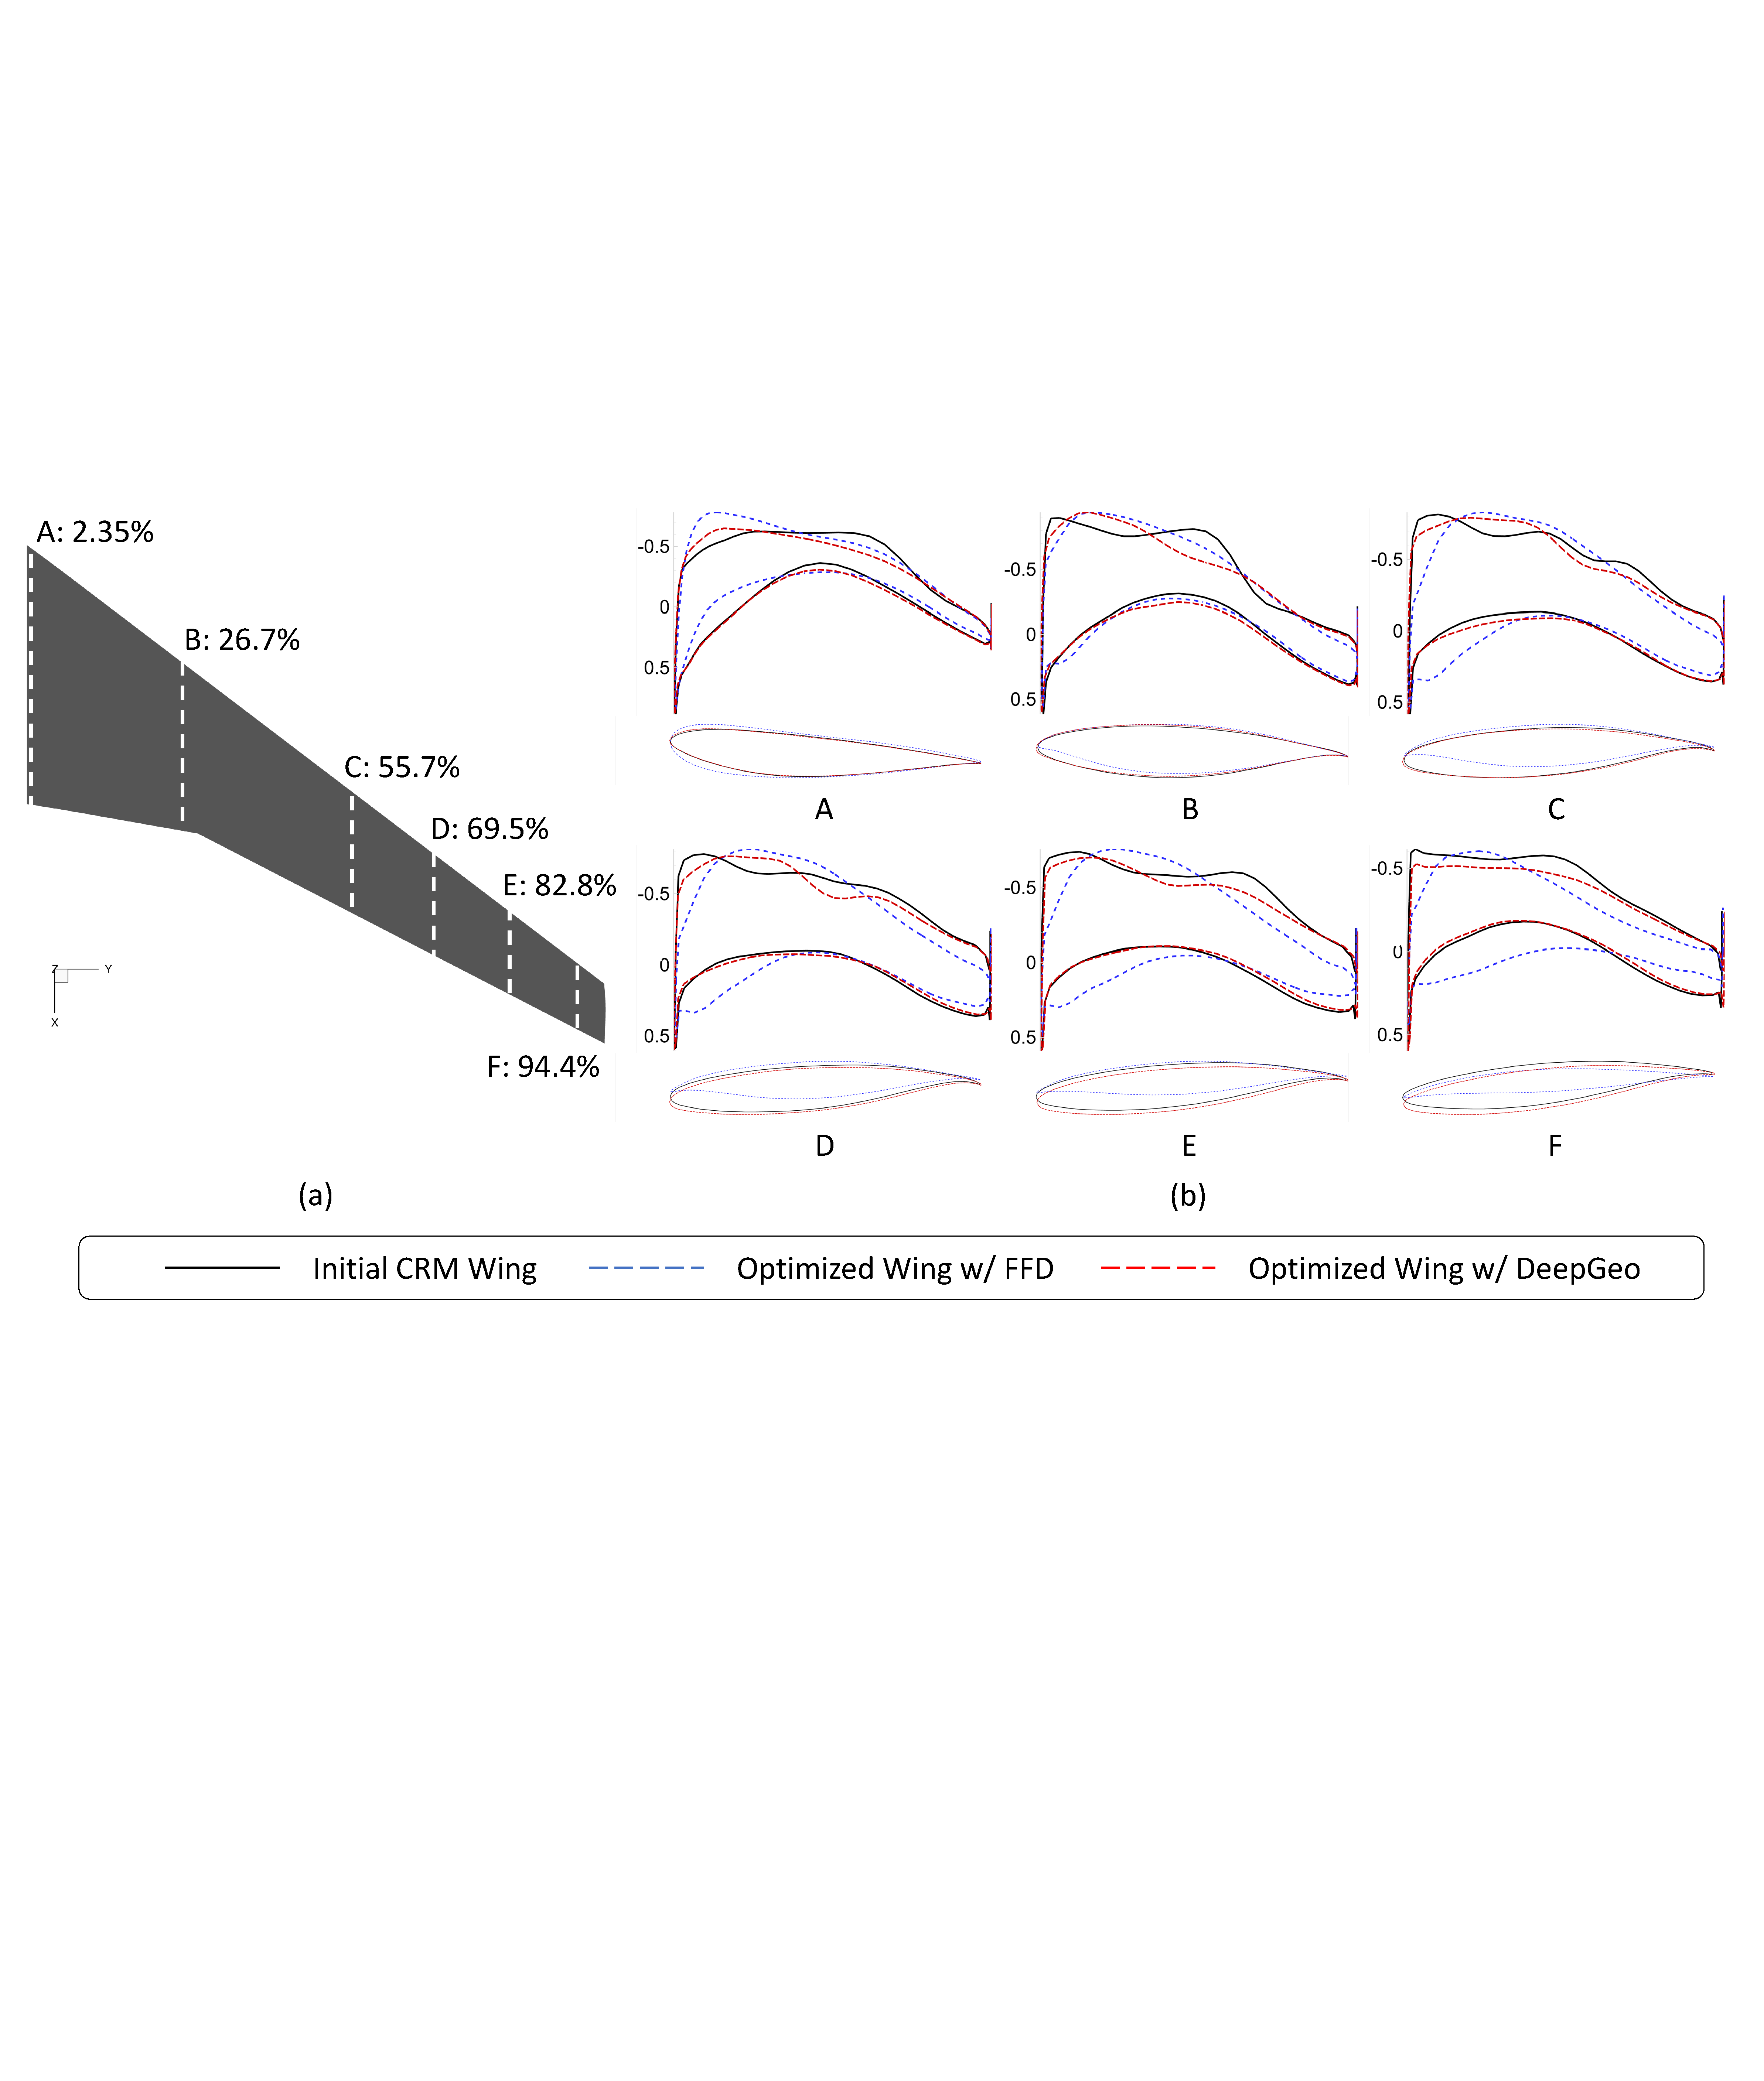
\includegraphics[width=1\linewidth]{chapter5/fig/crm_optim_slice.pdf}
    \end{center}
    \caption{
        \small A comparison of Case Study II on sliced geometries, including (a) the positions of slices, and (b) the shape variation and pressure coefficient distribution of each slice.
    }
    \label{ch5:fig:cs2_slice}
\end{figure}

Comparative quantitative results are presented in Tab.\ref{ch5:tab:crm_result}. The FFD results were obtained after extensive tuning, while DeepGeo achieved its results without requiring any parameter adjustments. 
The difference in the optimized drag coefficient $C_D$ is less than $0.5\%$. As noted by \citet{aa.Lyu2015}, even slight variations in FFD configuration can lead to increases of up to $2.4$ counts in the optimized drag coefficient.
Fig.~\ref{ch5:fig:cs2_history} shows the optimization history. The comparison with the history of the FFD-based optimization is provided in Appendix~\ref{ch5:sec:appendix_optim_history}.

Initially, DeepGeo parameterizes the CRM wing through self-initialization, similar to the approach used in the first case study on the 2D circle optimization. During the first 300 optimization iterations, the wing's lift-to-drag ratio ($L/D$) increases from $22.5$ to $23.8$.
Once the optimization converges, the partially optimized wing is reparameterized by self-initializing a new DeepGeo model.
The optimization continues after that.
The $L/D$ ratio reaches a maximum of $25.0$ before gradually decreasing, with the optimal result observed at the $320\text{th}$ iteration. The drag coefficient $C_D$ has been reduced by $10.9\%$.

In Fig.~\ref{ch5:fig:cs2_cp}, we compare the pressure distributions and shock wave patterns for both parameterization approaches. 
The shock waves are substantially reduced in both optimized results. The parallel alignment of pressure contour lines in both cases indicates improved aerodynamic performance, though they exhibit evident differences.
Fig.~\ref{ch5:fig:cs2_slice} compares 2D slices of the optimized wings at various locations along the wingspan. In terms of the constraint preservation, all six sectional slices across the span of DeepGeo's optimization result satisfy the $25\%$ original thickness constraint. FFD and DeepGeo yield distinct shapes: FFD results display very sharp leading edges and significant thickness variations along the span, while DeepGeo’s results show smaller deviations from the initial shape. The leading edges are less sharp, the trailing edges better adhere to geometric constraints, and the wing tips remain sufficiently thick so avoid extreme thinning.

The final design obtained with DeepGeo lies in a narrow design space close to the baseline geometry, which may be due to local convergence within the high-dimensional gradient-based optimization process under restrictive geometric constraints. 
The optimized shape tends to generate relatively smaller modifications of the initial design.
%However, this phenomenon is preferable for industry applications, as it preserves off-design performance with only minor modifications from the initial design, facilitating robust performance under different operating conditions. 
In contrast, the FFD-based optimization aggressively reduces the leading edge thickness to minimize on-design drag, potentially compromising low-speed aerodynamic performance~\cite{aa.Li2019} critical for landing and takeoff. Thus, DeepGeo’s approach is beneficial when starting from a good conceptual design, yielding a more controlled ASO pipeline with minimal adjustments.

In summary, DeepGeo achieves comparable aerodynamic performance to the best manually tuned FFD-based method with a simpler, less labor-intensive setup. Its ability to reduce the need for extensive tuning makes it an effective and practical choice for industrial aerodynamic optimization.